\subsection{Riepilogo}
\subsubsection{Ore totali}
\subsubsubsection{Suddivisione lavoro}
La seguente tabella riporta il totale delle ore del progetto,  comprese le ore di investimento e quelle rendicontate a carico del committente:
\begin{table}[!htbp]
\begin{center}
\rowcolors{2}{gray!25}{white}
\renewcommand{\arraystretch}{1.25}
\begin{tabular}{ m{0.20\textwidth}<{\centering}  m{0.06\textwidth}<{\centering} m{0.06\textwidth}<{\centering} m{0.06\textwidth}<{\centering}  m{0.06\textwidth}<{\centering}  m{0.06\textwidth}<{\centering}  m{0.06\textwidth}<{\centering}  m{0.20\textwidth}<{\centering}   }
	\rowcolor{darkblue}
	\textcolor{white}{\textbf{Componente}} &\textcolor{white}{\textbf{Re}}&\textcolor{white}{\textbf{Pt}}&\textcolor{white}{\textbf{An}}&\textcolor{white}{\textbf{Am}}&\textcolor{white}{\textbf{Pr}}&\textcolor{white}{\textbf{Ve}}&\textcolor{white}{\textbf{Ore complessive}}\\ 
	Edoardo Pavan & 0 & 0 & 0 & 0 & 0 & 1 & 1 \\	
	
	Francesco Protopapa & 1 & 0 & 0 & 1 & 0 & 1 & 3 \\

	Greta Cavedon & 1 & 1 & 0 & 1 & 0 & 1 & 4 \\
	
	Luciano Wu & 0 & 5 & 0 & 0 & 0 & 0 &5 \\
	
	Matteo Basso & 0 & 2 & 0 & 1 & 0 & 1 & 4 \\
	
	Michele Gatto & 0 & 4 & 0 & 0 & 0 & 0 & 4 \\
	
	Pietro Villatora & 1 & 4 & 0 & 0 & 0 & 0 & 5 \\
	
	\textbf{Ore totali ruolo} & 3 & 16 & 0 & 3 & 0 & 4 & 26 \\

\end{tabular}
\caption{Distribuzione delle ore totali per ogni componente del gruppo}
\end{center}
\end{table}

La tabella può essere rappresentata anche in forma visiva dal seguente grafico:
\begin{figure}[!h]
\centering
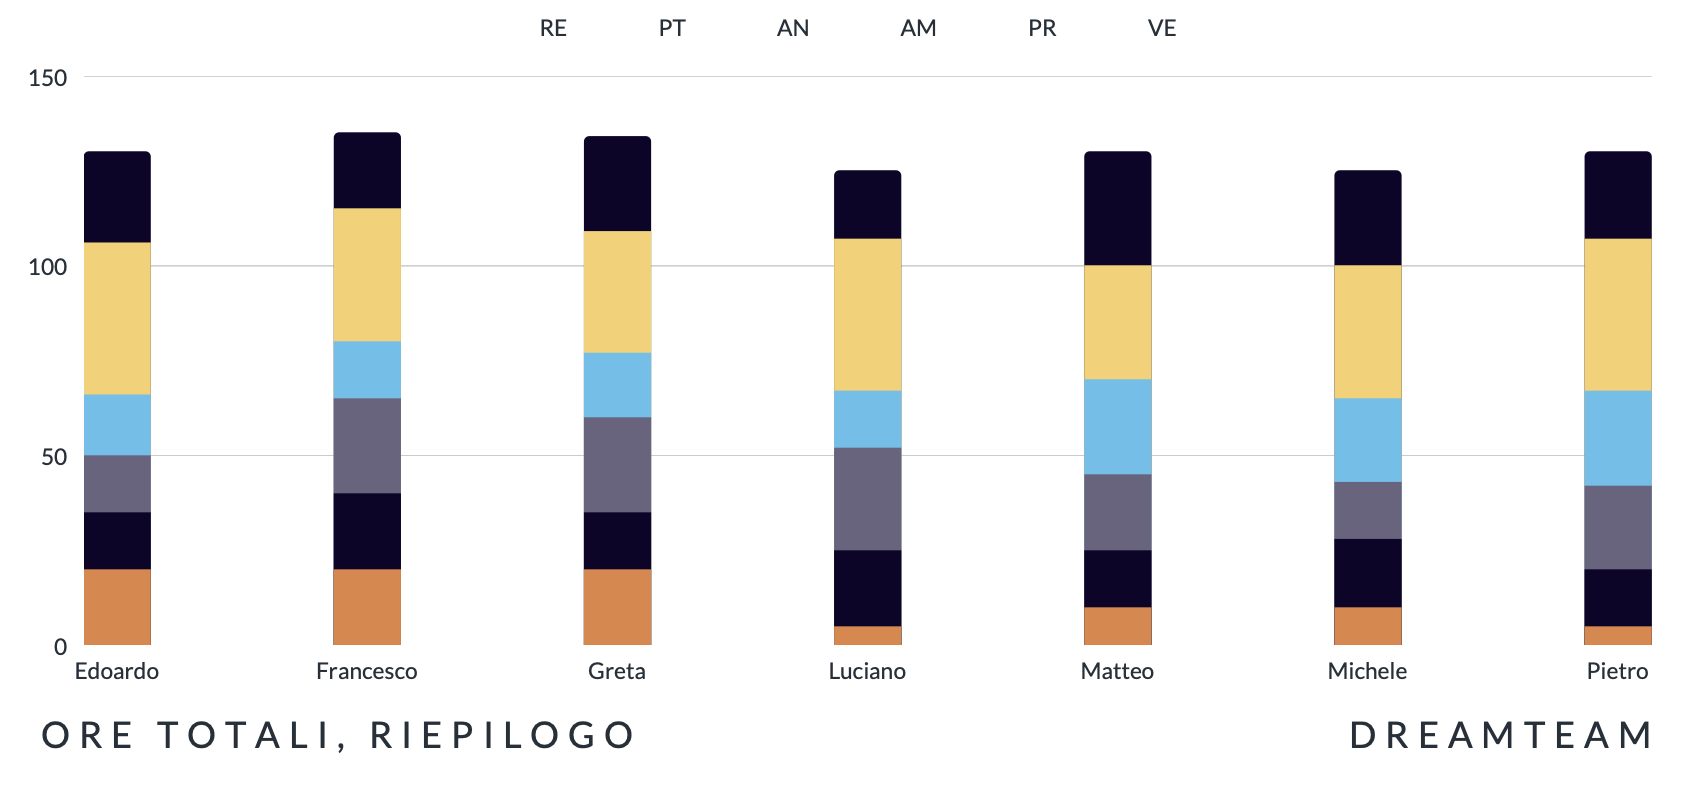
\includegraphics[scale=0.65]{Sezioni/SezioniPreventivo/grafici/Riepilogo_ore_totali.png}
\caption{Istogramma della ripartizione delle ore totali di investimento e rendicontate}
\end{figure}

\subsubsubsection{Prospetto economico}
La seguente tabella rappresenta le ore totali dedicate ad ogni ruolo e il costo in euro:

\begin{table}[!htbp]
\begin{center}
\rowcolors{2}{gray!25}{white}
\renewcommand{\arraystretch}{1.5}
\begin{tabular}{ m{0.3\textwidth}<{\centering}  m{0.2\textwidth}<{\centering} m{0.2\textwidth}<{\centering}}
	\rowcolor{darkblue}
	\textcolor{white}{\textbf{Ruolo}}&\textcolor{white}{\textbf{Totale ore}}&\textcolor{white}{\textbf{Costo totale (\euro)}}\\ 

	Responsabile  & 3 & 90 \\	
	
	Progettista & 16 & 400 \\
	
	Analista & 0 & 0 \\

	Amministratore & 3 & 60 \\
	
	Programmatore & 0 & 0 \\
	
	Verificatore & 4 & 60 \\
	
	\textbf{Totale} & 26 & 610 \\
	
\end{tabular}
\caption{Prospetto dei costi totali delle ore totali di investimento e rendicontate}
\end{center}
\end{table}

La tabella può essere rappresentata anche in forma visiva dal seguente aerogramma:
\begin{figure}[!h]
\centering
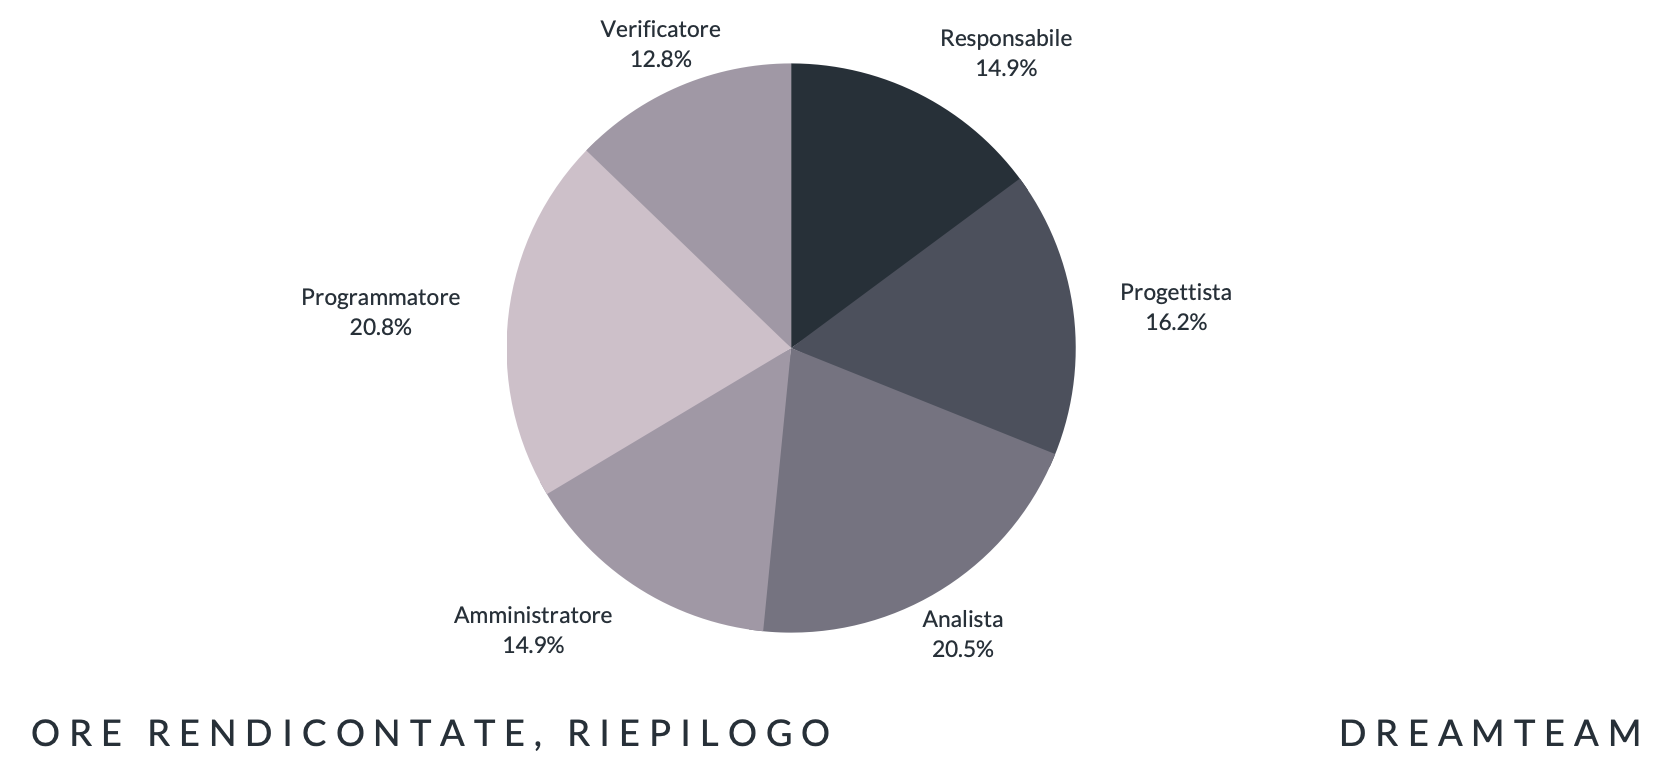
\includegraphics[scale=0.65]{Sezioni/SezioniPreventivo/grafici/Riepilogo_ore_totali_costi.png}
\caption{Grafico a torta della ripartizione per ruolo delle ore totali di investimento e rendicontate}
\end{figure}



\subsubsection{Ore rendicontate}
\subsubsubsection{Suddivisione lavoro}
La seguente tabella riporta le ore rendicontate: 
\begin{table}[!htbp]
\begin{center}
\rowcolors{2}{gray!25}{white}
\renewcommand{\arraystretch}{1.25}
\begin{tabular}{ m{0.20\textwidth}<{\centering}  m{0.06\textwidth}<{\centering} m{0.06\textwidth}<{\centering} m{0.06\textwidth}<{\centering}  m{0.06\textwidth}<{\centering}  m{0.06\textwidth}<{\centering}  m{0.06\textwidth}<{\centering}  m{0.20\textwidth}<{\centering}   }
	\rowcolor{darkblue}
	\textcolor{white}{\textbf{Componente}} &\textcolor{white}{\textbf{Re}}&\textcolor{white}{\textbf{Pt}}&\textcolor{white}{\textbf{An}}&\textcolor{white}{\textbf{Am}}&\textcolor{white}{\textbf{Pr}}&\textcolor{white}{\textbf{Ve}}&\textcolor{white}{\textbf{Ore complessive}}\\ 
	Edoardo Pavan & 10 & 15 & 10 & 13 & 32 & 20 & 100 \\	
	
	Francesco Protopapa & 10 & 10 & 20 & 5 & 35 & 20 & 100 \\

	Greta Cavedon & 15 & 10 & 20 & 4 & 26 & 25 & 100 \\
	
	Luciano Wu & 5 & 20 & 20 & 4 & 31 & 15 & 95 \\
	
	Matteo Basso & 5 & 15 & 15 & 10 & 25 & 20 & 90 \\
	
	Michele Gatto & 10 & 15 & 5 & 12 & 28 & 20 & 90 \\
	
	Pietro Villatora & 5 & 15 & 10 & 12 & 38 & 20 & 100 \\
	
	\textbf{Ore totali ruolo} & 60 & 100 & 100 & 60 & 215 & 140 & 675 \\

\end{tabular}
\caption{Distribuzione delle ore rendicontate}
\end{center}
\end{table}

La tabella può essere rappresentata anche in forma visiva dal seguente grafico:
\begin{figure}[!h]
\centering
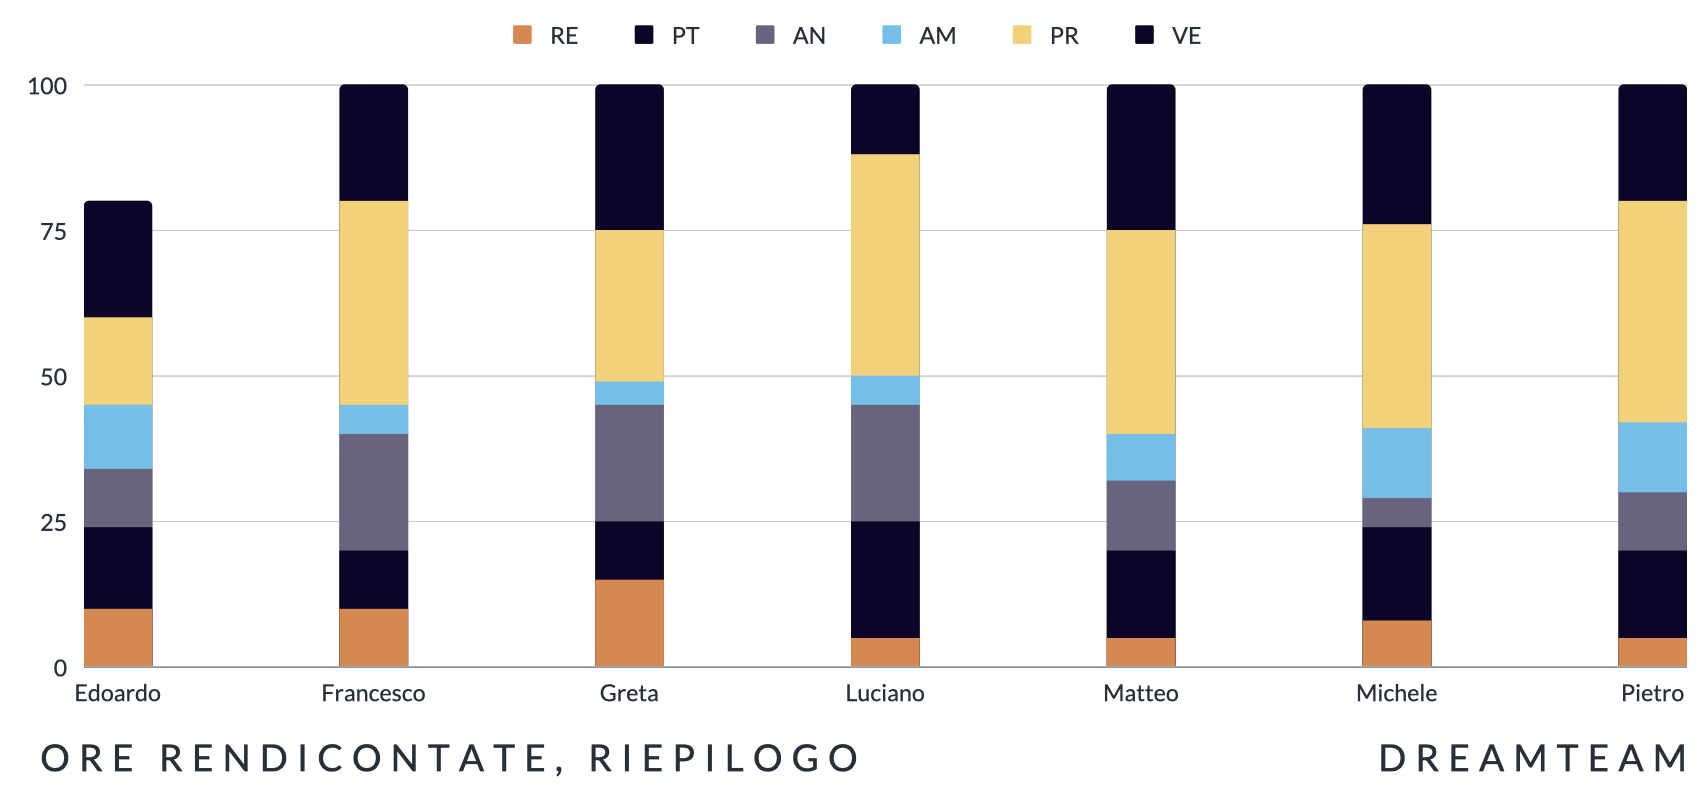
\includegraphics[scale=0.65]{Sezioni/SezioniPreventivo/grafici/Riepilogo_ore_rendicontate.png}
\caption{Istogramma della ripartizione delle ore rendicontate}
\end{figure}

\subsubsubsection{Prospetto economico}
La seguente tabella rappresenta le ore totali dedicate ad ogni ruolo e il costo in euro:

\begin{table}[!htbp]
\begin{center}
\rowcolors{2}{gray!25}{white}
\renewcommand{\arraystretch}{1.5}
\begin{tabular}{ m{0.3\textwidth}<{\centering}  m{0.2\textwidth}<{\centering} m{0.2\textwidth}<{\centering}}
	\rowcolor{darkblue}
	\textcolor{white}{\textbf{Ruolo}}&\textcolor{white}{\textbf{Totale ore}}&\textcolor{white}{\textbf{Costo totale (\euro)}}\\ 

	Responsabile  & 60 & 1800 \\	
	
	Progettista & 100 & 2500 \\
	
	Analista & 100 & 2500 \\

	Amministratore & 60 & 1200 \\
	
	Programmatore & 215 & 3225 \\
	
	Verificatore & 140 & 2100 \\
	
	\textbf{Totale} & 675 & 13325 \\
	
\end{tabular}
\caption{Prospetto dei costi totali delle ore rendicontate}
\end{center}
\end{table}

La tabella può essere rappresentata anche in forma visiva dal seguente aerogramma:
\begin{figure}[!h]
\centering
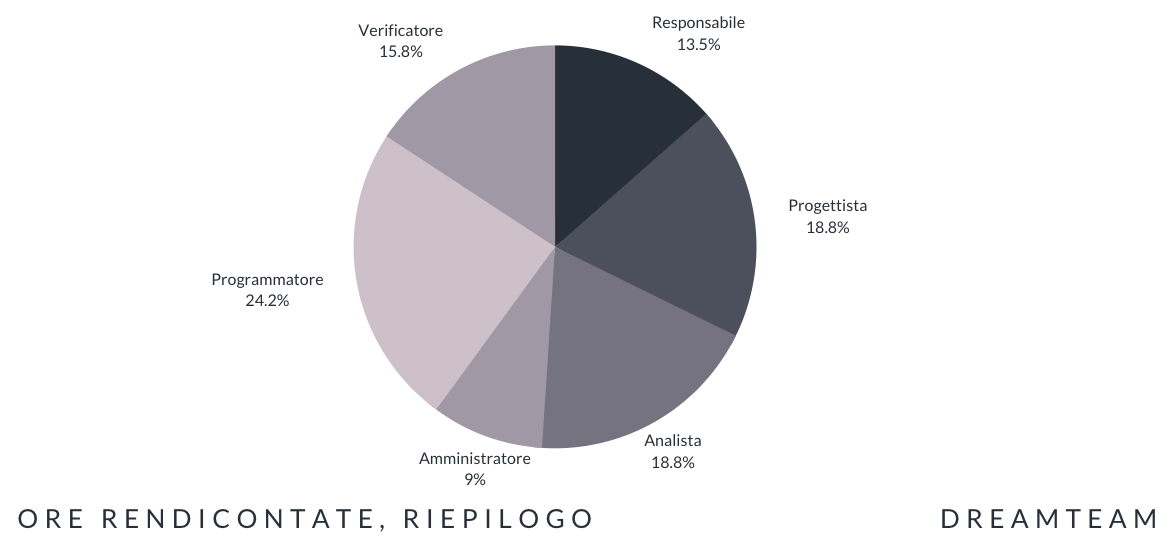
\includegraphics[scale=0.65]{Sezioni/SezioniPreventivo/grafici/Riepilogo_ore_rendicontate_costi.png}
\caption{Grafico a torta della ripartizione per ruolo delle ore rendicontate}
\end{figure}